\section{Methodology}
\label{sec:methodology}

This section details our implementation methodology, covering system architecture, data generation strategy, training pipeline, evaluation framework, and prompt engineering. Our approach follows a staged validation strategy, with each stage building on validated success from the previous stage.

\subsection{System Architecture}
\label{subsec:system_architecture}

Our system follows a layered architecture (see Figure~\ref{fig:architecture}) that separates concerns between CLI interface, application logic, domain models, and infrastructure adapters.

\begin{figure}[h]
\centering
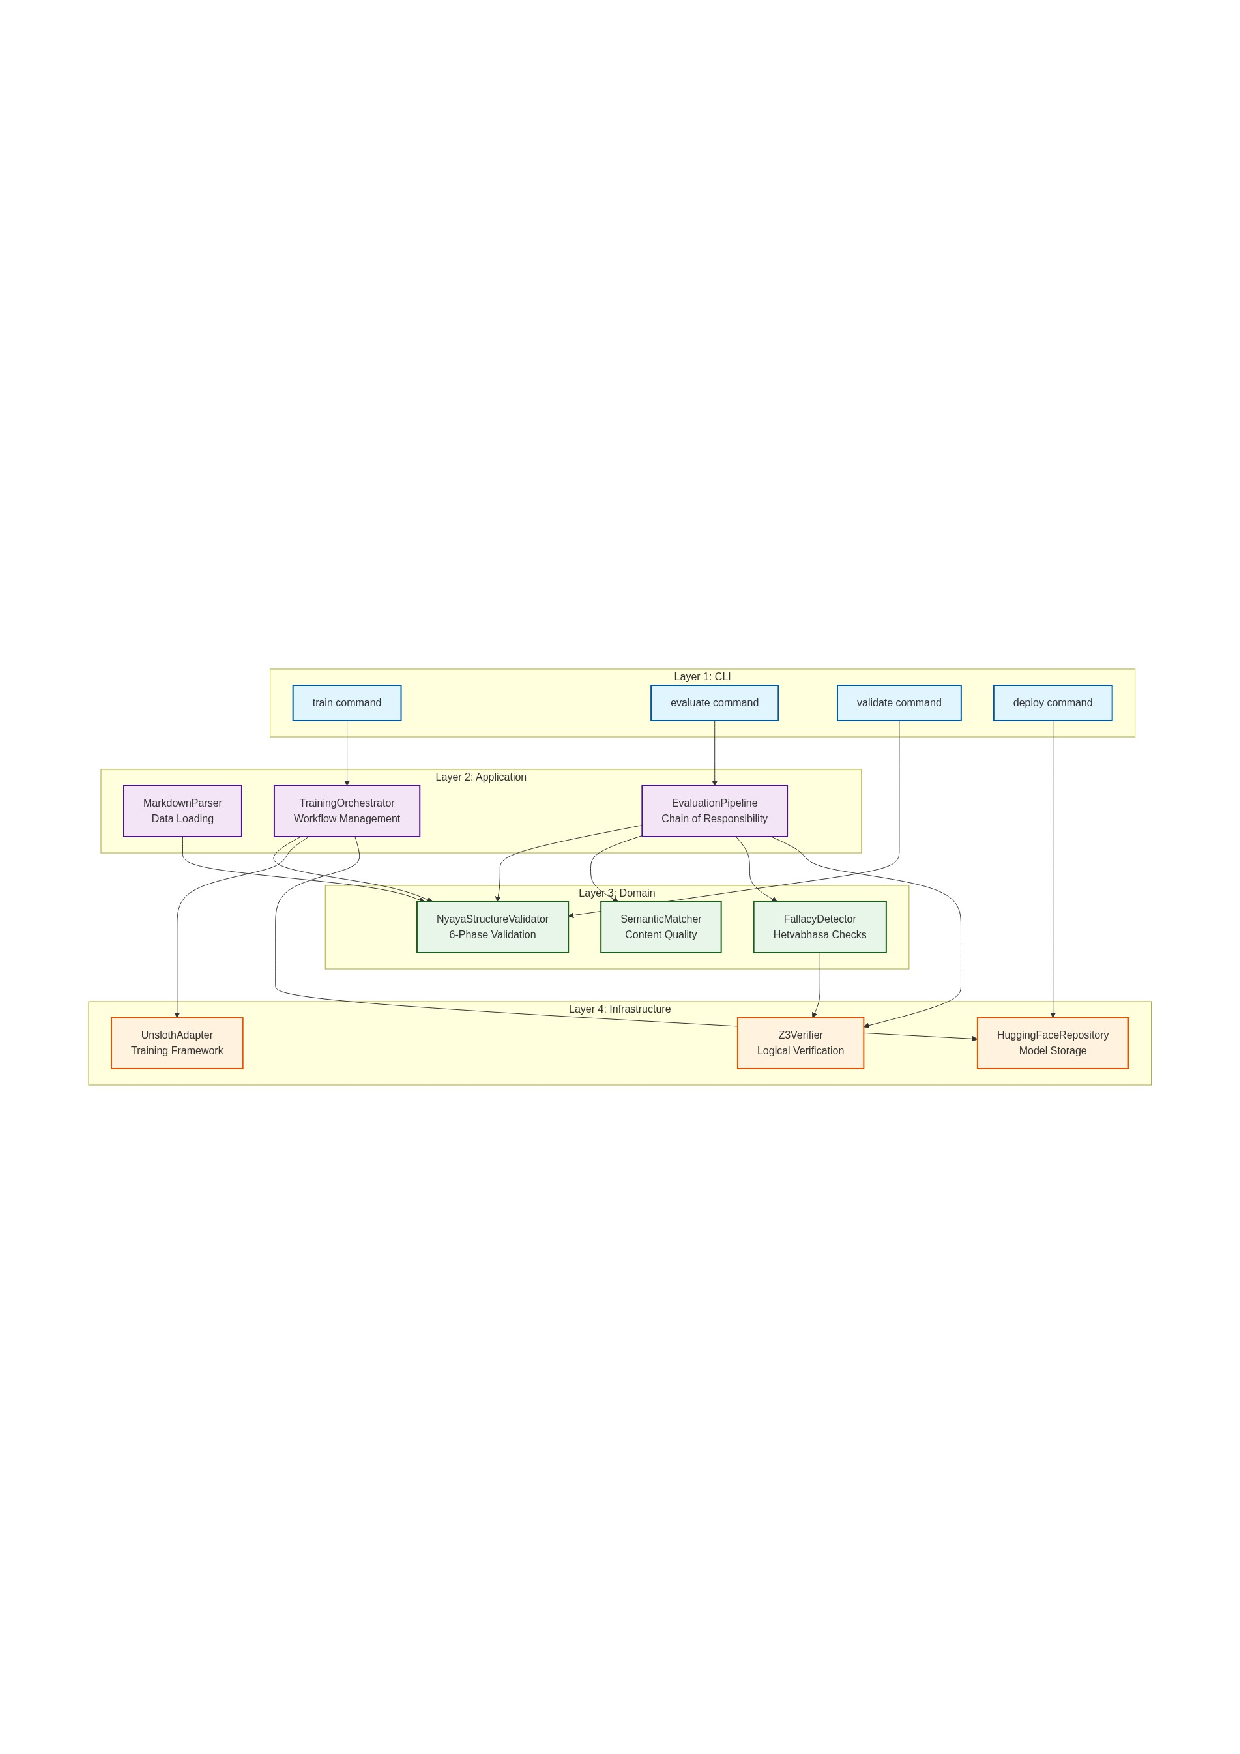
\includegraphics[width=0.9\textwidth]{figures/architecture.pdf}
\caption{System architecture showing layered design: CLI $\rightarrow$ Application $\rightarrow$ Domain $\rightarrow$ Infrastructure. Key components include MarkdownParser, NyayaStructureValidator, EvaluationPipeline, and Z3Verifier.}
\label{fig:architecture}
\end{figure}

\textbf{Layered design}:

\begin{enumerate}
    \item \textbf{CLI Layer} (\texttt{src/pramana/cli/}): Command-line interface using Typer, providing \texttt{train}, \texttt{evaluate}, \texttt{validate}, and \texttt{data} commands.
    \item \textbf{Application Layer} (\texttt{src/pramana/application/}):
    \begin{itemize}
        \item \texttt{data/parser.py}: \texttt{MarkdownParser} converts markdown files with YAML frontmatter into \texttt{NyayaExample} domain models
        \item \texttt{evaluation/pipeline.py}: \texttt{EvaluationPipeline} orchestrates multi-tier evaluation using chain-of-responsibility pattern
        \item \texttt{training/}: Training orchestrators for supervised fine-tuning
    \end{itemize}
    \item \textbf{Domain Layer} (\texttt{src/pramana/domain/}):
    \begin{itemize}
        \item \texttt{validators/structure.py}: \texttt{NyayaStructureValidator} validates 6-phase completeness, Pramana sources, syllogism integrity
        \item \texttt{models/nyaya_example.py}: Domain models for NyayaExample, Samshaya, Pramana, PanchaAvayava, Tarka, Hetvabhasa, Nirnaya
    \end{itemize}
    \item \textbf{Infrastructure Layer} (\texttt{src/pramana/infrastructure/}):
    \begin{itemize}
        \item \texttt{ml/unsloth_adapter.py}: Adapter for Unsloth's FastLanguageModel API
        \item \texttt{verification/z3_verifier.py}: \texttt{Z3Verifier} for SMT-LIB validation of formal logic problems
    \end{itemize}
\end{enumerate}

This architecture enables clean separation of concerns, testability, and extensibility for future stages (e.g., GRPO training, multi-agent protocols).

\subsection{Data Generation Strategy}
\label{subsec:data_generation}

We follow a seed-and-expand strategy, prioritizing quality over quantity. All examples are human-verified before inclusion in training datasets.

\subsubsection{Stage 0: Proof of Concept}

\textbf{Dataset size}: 20 manual seed examples

\textbf{Problem type distribution}:

\begin{table}[h]
\centering
\small
\begin{tabular}{lcc}
\toprule
Problem Type & Count & Example IDs \\
\midrule
Constraint Satisfaction & 4 & pramana-001, 006, 007, 008 \\
Boolean SAT & 4 & pramana-002, 009, 010, 011 \\
Transitive Reasoning & 4 & pramana-003, 012, 013, 014 \\
Set Membership & 4 & pramana-004, 015, 016, 017 \\
Multi-Step Deduction & 4 & pramana-005, 018, 019, 020 \\
\bottomrule
\end{tabular}
\caption{Stage 0 seed example distribution by problem type. All examples manually created and validated.}
\label{tab:stage0_distribution}
\end{table}

\textbf{Quality assurance}: All 20 examples human-verified for:
\begin{itemize}
    \item All 6 phases present and in correct order
    \item Pratyaksha contains only observable facts (no inferences)
    \item Each Udaharana contains ``Wherever X, there is Y'' universal rule
    \item Tarka actually tests conclusion via reductio ad absurdum (not tautological)
    \item All 5 Hetvabhasa types explicitly checked
    \item Ground truth answer is verifiable and correct
\end{itemize}

\subsubsection{Stage 1: Minimum Viable Reasoner}

\textbf{Dataset size}: 55 examples total (20 Stage 0 + 35 new Stage 1 examples)

\textbf{Stage 1 additions}: 35 new examples including:
\begin{itemize}
    \item 30 positive examples: 6 each of constraint satisfaction, Boolean SAT, transitive reasoning, set membership, multi-step deduction
    \item 5 negative/contrastive examples: Intentionally flawed examples demonstrating common errors:
    \begin{itemize}
        \item \texttt{stage1-neg-001-pratyaksha.md}: Pratyaksha contamination (includes inferred facts)
        \item \texttt{stage1-neg-002-udaharana.md}: Missing universal rule in Udaharana
        \item \texttt{stage1-neg-003-tarka.md}: Circular Tarka (tautological)
        \item \texttt{stage1-neg-004-hetvabhasa.md}: Incomplete Hetvabhasa (missing fallacy checks)
        \item \texttt{stage1-neg-005-nirnaya.md}: False certainty (claims definitive knowledge without proper grounding)
    \end{itemize}
\end{itemize}

\textbf{Quality assurance}: All 55 examples human-verified. Negative examples labeled with \texttt{negative\_example: true} in YAML frontmatter for potential contrastive learning or DPO-style preference training in future stages.

\textbf{Training data format}: Examples converted to JSONL format (\texttt{data/training/stage\_1.jsonl}) with:
\begin{itemize}
    \item \texttt{instruction}: Problem statement
    \item \texttt{input}: Empty string (reserved for future)
    \item \texttt{output}: Full Nyaya reasoning trace from \samshaya{} to \nirnaya{}
\end{itemize}

\subsection{Training Pipeline}
\label{subsec:training_pipeline}

We use supervised fine-tuning (SFT) with QLoRA (4-bit quantization) via Unsloth for efficient training on DGX Spark infrastructure.

\subsubsection{Stage 0: Proof of Concept}

\textbf{Base model}: \texttt{unsloth/Llama-3.2-3B-Instruct-bnb-4bit}

\textbf{Rationale}: Small model (3B parameters) sufficient for proof-of-concept to validate that Nyaya structure is learnable. Chosen for fast iteration and lower memory requirements.

\textbf{LoRA configuration}:
\begin{itemize}
    \item Rank: 64, Alpha: 64
    \item Target modules: All attention (\texttt{q\_proj}, \texttt{k\_proj}, \texttt{v\_proj}, \texttt{o\_proj}) and FFN (\texttt{gate\_proj}, \texttt{up\_proj}, \texttt{down\_proj})
    \item LoRA dropout: 0 (optimized by Unsloth)
    \item Gradient checkpointing: \texttt{unsloth} (30\% VRAM reduction)
\end{itemize}

\textbf{Training hyperparameters}:

\begin{table}[h]
\centering
\small
\begin{tabular}{lc}
\toprule
Parameter & Value \\
\midrule
Epochs & 30 \\
Learning rate & $2 \times 10^{-5}$ \\
Batch size (per device) & 2 \\
Gradient accumulation steps & 4 \\
Effective batch size & 8 \\
Sequence length & 4096 tokens \\
Optimizer & \texttt{adamw\_8bit} \\
Precision & bf16 \\
Warmup steps & 4 \\
Train/validation split & 80/20 (16 train, 4 val) \\
\bottomrule
\end{tabular}
\caption{Stage 0 training hyperparameters. High LoRA rank (64) and long sequence length (4096) chosen to embed new reasoning paradigm.}
\label{tab:stage0_hyperparams}
\end{table}

\textbf{Hardware}: Single A100 (40GB) on NVIDIA DGX Spark

\textbf{Training time}: $\sim$4--6 GPU-hours

\textbf{Format enforcement}: Explicit format instructions and template injected into user prompt (see Section~\ref{subsec:prompt_engineering}).

\subsubsection{Stage 1: Minimum Viable Reasoner}

\textbf{Base model}: \texttt{unsloth/DeepSeek-R1-Distill-Llama-8B-bnb-4bit}

\textbf{Rationale}: DeepSeek-R1-Distill-Llama-8B has pre-trained reasoning traces, making it better suited for learning structured reasoning. Larger capacity (8B vs 3B) enables more complex reasoning patterns.

\textbf{LoRA configuration}:
\begin{itemize}
    \item Rank: 64, Alpha: 64
    \item Target modules: Same as Stage 0 (all attention + FFN)
    \item LoRA dropout: 0
    \item Gradient checkpointing: \texttt{unsloth}
\end{itemize}

\textbf{Training hyperparameters}:

\begin{table}[h]
\centering
\small
\begin{tabular}{lc}
\toprule
Parameter & Value \\
\midrule
Epochs & 10 \\
Learning rate & $2 \times 10^{-5}$ \\
Batch size (per device) & 1 \\
Gradient accumulation steps & 4 \\
Effective batch size & 4 \\
Sequence length & 4096 tokens \\
Optimizer & \texttt{adamw\_8bit} \\
Precision & bf16 \\
Warmup steps & 4 \\
Train/validation split & 80/20 (44 train, 11 val) \\
\bottomrule
\end{tabular}
\caption{Stage 1 training hyperparameters. Conservative learning rate preserves pre-trained reasoning capabilities.}
\label{tab:stage1_hyperparams}
\end{table}

\textbf{Hardware}: Single A100 (40GB) on NVIDIA DGX Spark

\textbf{Training observability}: \texttt{NyayaMetricsCallback} (implemented in \texttt{src/pramana/application/training/callbacks.py}) tracks:
\begin{itemize}
    \item Format adherence (fraction of phases present)
    \item Phase count (0--6)
    \item Syllogism count per solution
\end{itemize}

Metrics logged to Weights \& Biases during training for real-time monitoring.

\subsection{Evaluation Framework}
\label{subsec:evaluation}

We employ a three-tier evaluation framework that progressively validates structural correctness, content quality, and logical validity.

\subsubsection{Tier 1: Structural Validation}

\textbf{Purpose}: Fast automated checks for format compliance

\textbf{Checks} (implemented in \texttt{NyayaStructureValidator}):
\begin{itemize}
    \item All 6 phases present and in correct order
    \item Pramana completeness: All 4 types (Pratyaksha, Anumana, Upamana, Shabda) present
    \item Syllogism integrity: $\geq$1 syllogism with all 5 members (Pratijna, Hetu, Udaharana, Upanaya, Nigamana)
    \item Udaharana universal rule: Must contain ``Wherever X, there is Y'' structure
    \item Hetvabhasa completeness: All 5 fallacy types checked
\end{itemize}

\textbf{Output}: Binary pass/fail (1.0 if valid, 0.0 if invalid)

\textbf{Stage 0 results}: 100\% format adherence (2/2 test examples parseable with all 6 phases)

\textbf{Stage 1 results}: 40\% format adherence (4/10 test examples parseable). Primary failure modes: missing Hetvabhasa section (2), missing Nirnaya section (1), invalid doubt types (2).

\subsubsection{Tier 2: Content Quality Scoring}

\textbf{Purpose}: LLM-as-judge evaluation using explicit Nyaya rubric

\textbf{Implementation}: \texttt{Tier2LLMJudgeHandler} (in \texttt{src/pramana/application/evaluation/llm_judge.py}) uses GPT-4 or Claude with structured rubric scoring each phase 0--10:

\begin{itemize}
    \item Samshaya appropriateness: Correct doubt type classification?
    \item Pratyaksha validity: Only observables (no inferred facts)?
    \item Anumana correctness: Actual logical inferences (not restatements)?
    \item Upamana relevance: Appropriate analogies?
    \item Shabda correctness: Valid universal principles?
    \item Pancha Avayava quality: Universal rules in Udaharana?
    \item Tarka meaningfulness: Actually tests conclusion (not tautological)?
    \item Hetvabhasa thoroughness: All 5 types checked?
    \item Nirnaya definitiveness: Appropriate confidence level?
\end{itemize}

\textbf{Scoring thresholds}:
\begin{itemize}
    \item $\geq$0.85 (77/90+): AUTO-ACCEPT
    \item 0.70--0.84 (63--76/90): MANUAL\_REVIEW
    \item $<$0.70 ($<$63/90): REJECT
\end{itemize}

\textbf{Status}: Tier 2 evaluation not run for Stage 0/1 held-out test sets (planned for Stage 2 synthetic data quality control).

\subsubsection{Tier 3: Ground Truth Matching}

\textbf{Purpose}: Verify answer correctness

\textbf{Methods}:
\begin{itemize}
    \item \textbf{Exact match}: String equality (overly strict, fails on semantically correct answers)
    \item \textbf{Normalized match}: Case-insensitive, punctuation-normalized comparison
    \item \textbf{Semantic similarity}: Cosine similarity using sentence-transformers embeddings
\end{itemize}

\textbf{Stage 0 results}: 0\% exact match (0/2), but 100\% semantic correctness (both answers semantically correct despite failing exact string matching)

\textbf{Stage 1 results}: 100\% semantic correctness (10/10), demonstrating strong reasoning content despite format adherence issues

\subsubsection{Z3 Verification (Future Work)}

For formal logic problems (constraint satisfaction, Boolean SAT), we plan to implement runtime Z3 SMT-LIB verification:
\begin{itemize}
    \item Parse Pratijna/Hetu/Udaharana from model output
    \item Autoformalize to Z3 SMT-LIB format
    \item Execute Z3 solver to verify logical validity
    \item If invalid, inject error feedback and trigger model self-correction
\end{itemize}

\textbf{Status}: Z3Verifier infrastructure exists (\texttt{src/pramana/infrastructure/verification/z3_verifier.py}) but not integrated into evaluation pipeline for Stage 0/1.

\subsection{Prompt Engineering}
\label{subsec:prompt_engineering}

Format enforcement via explicit prompt engineering was critical for Stage 0 success. The initial training run (without format enforcement) achieved 0\% format adherence; the corrected run (with explicit format instructions) achieved 100\% format adherence.

\subsubsection{System Prompt}

\textbf{Template}: ``You are a Nyaya reasoning engine. Follow the exact output format provided.''

This establishes the model's role and emphasizes format compliance.

\subsubsection{Format Instructions}

Explicit list of required sections in strict order:

\begin{verbatim}
Required section order:
1) ## Samshaya (Doubt Analysis)
2) ## Pramana (Sources of Knowledge)
3) ## Pancha Avayava (5-Member Syllogism)
4) ## Tarka (Counterfactual Reasoning)
5) ## Hetvabhasa (Fallacy Check)
6) ## Hetvabhasa (Fallacy Check)

CRITICAL:
- Your response MUST start with: "## Samshaya (Doubt Analysis)"
- Copy the template exactly and fill in every field.
- Do not add any text before the first header or after the final field.
\end{verbatim}

\subsubsection{Template Injection}

A skeletal markdown template is injected into the user prompt, showing the exact structure expected:

\begin{verbatim}
## Samshaya (Doubt Analysis)
**Doubt Type**:
**Justification**:

---

## Pramana (Sources of Knowledge)
### Pratyaksha (Direct Perception)
- 
### Anumana (Inference)
- 
### Upamana (Comparison)
- 
### Shabda (Testimony)
- 

---

## Pancha Avayava (5-Member Syllogism)
### Syllogism 1: 
**Pratijna (Thesis)**:
**Hetu (Reason)**:
**Udaharana (Universal + Example)**:
**Upanaya (Application)**:
**Nigamana (Conclusion)**:

---

## Tarka (Counterfactual Reasoning)
**Hypothesis**:
**Consequence**:
**Analysis**:
**Resolution**:

---

## Hetvabhasa (Fallacy Check)
Check for Savyabhichara: 
Check for Viruddha: 
Check for Asiddha: 
Check for Satpratipaksha: 
Check for Badhita: 

---

## Nirnaya (Ascertainment)
**Final Answer**:
**Justification**:
**Confidence**:
\end{verbatim}

\subsubsection{Critical Constraint}

\textbf{Response must start with}: ``## Samshaya (Doubt Analysis)''

This constraint prevents the model from adding introductory text or deviating from the expected format. Training examples are formatted to enforce this constraint, and the tokenizer's chat template (when available) preserves the structure.

\subsubsection{Format Validation During Training}

\texttt{FormatValidationCallback} (in \texttt{scripts/train\_stage0\_corrected.py}) monitors format adherence during training by:
\begin{itemize}
    \item Generating sample outputs on validation problems every N steps
    \item Checking phase presence via regex pattern matching
    \item Logging format adherence percentage
\end{itemize}

This enables early detection of format learning issues, though callback logs were not persisted to files in Stage 0/1 runs.
